Будем считать, что стена состоит из $10$ столбцов и строится за шесть действий. Все
приведенные интервалы включают границы. Изображения стены после каждого действия
представлены на рисунке ниже.

\begin{center}
\renewcommand{\arraystretch}{1.5}
\begin{tabular}{ |c|c|c|c| }
\hline
Действие & Вид & Интервал & Высота\\
\hline
0 & добавление & столбцы с 1 по 8 & 4 \\
\hline
1 & удаление & столбцы с 4 по 9 & 1 \\
\hline
2 & удаление & столбцы с 3 по 6 & 5 \\
\hline
3 & добавление & столбцы с 0 по 5 & 3 \\
\hline
4 & добавление & столбец 2 & 5 \\
\hline
5 & удаление & столбцы с 6 по 7 & 0 \\
\hline
\end{tabular}
\end{center}

Так как изначально все столбцы не содержат кирпичей, то после действия 0 каждый из
столбцов с номерами от 1 до 8 будет содержать по 4 кирпича, столбцы с номерами 0 и 9 будут
пустыми. После действия 1 в столбцах с номерами с 4 по 8 остается один кирпич, 9-й
столбец остается пустым. Столбцы с номерами с 0 по 3 лежат вне интервала и не меняются.
Действие 2 не меняет столбцы с номерами с 3 по 6, так как в них и так меньше пяти кирпичей.
После действия 3 количество кирпичей в столбцах с номерами 0, 4 и 5 увеличивается до 3.
После действия 4 во втором столбце становится пять кирпичей. За 5-е действие из столбцов с номерами 6 и 7 убираются все кирпичи.

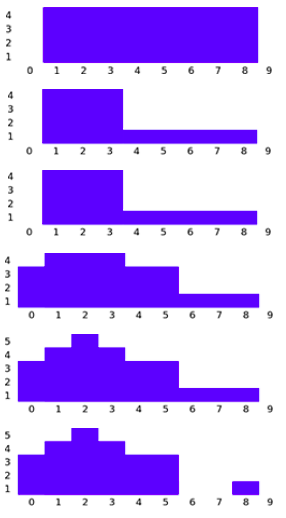
\includegraphics{1.png}